\chapter{全球时空感知:长期跟踪系统}\label{chap:globally}

\section{摘要}
尽管暹罗跟踪器已经取得了出色的性能,但是这些方法倾向于使用局部搜索机制,因此倾向于累积预测位置的不准确性,从而导致跟踪随时间的漂移,尤其是在长期跟踪情况下。为了解决这些问题,我们本着更快的RCNN的两阶段检测范例的精神,提出了一种暹罗跟踪器。这种新的跟踪器致力于基于全局感知机制来减少累积的不准确性并提高鲁棒性,该机制可在整个图像平面上及时在空间上检索目标。由于可以在此两阶段跟踪框架中启用非常深的网络进行特征学习,因此可以保证区分的能力。此外,我们还添加了基于CNN的轨迹预测模块,该模块利用目标的时间运动信息来减轻干扰因素的干扰。
这两个空间和时间模块利用高级外观信息和互补轨迹信息来提高跟踪的鲁棒性。全面的实验表明,所提出的基于全球时空知觉的跟踪系统的性能优于最先进的跟踪器。

\section{简介}
\label{sec:intro}

目标跟踪 \cite{Leang2018OnlineFO, Wang2019VisualOT, Zhang2018UsingFL} 是计算机视觉领域中一个具有挑战性的问题,该目标旨在建立连续视频序列中待跟踪目标的位置关系。
流行的暹罗跟踪器 \cite{SiamFC, SiamRPN, Wang2018SiamMask} 通常基于本地搜索机制: \HL{搜索目标} 在以前一帧的目标位置为中心的小邻域中确定 \HL{其当前位置}.
如果目标仅在两个相邻帧之间具有较小的位移,则此机制起作用。这在另一个方面也带来了好处,避免了来自干扰因素的干扰。

\begin{figure}[t]
    \centering
    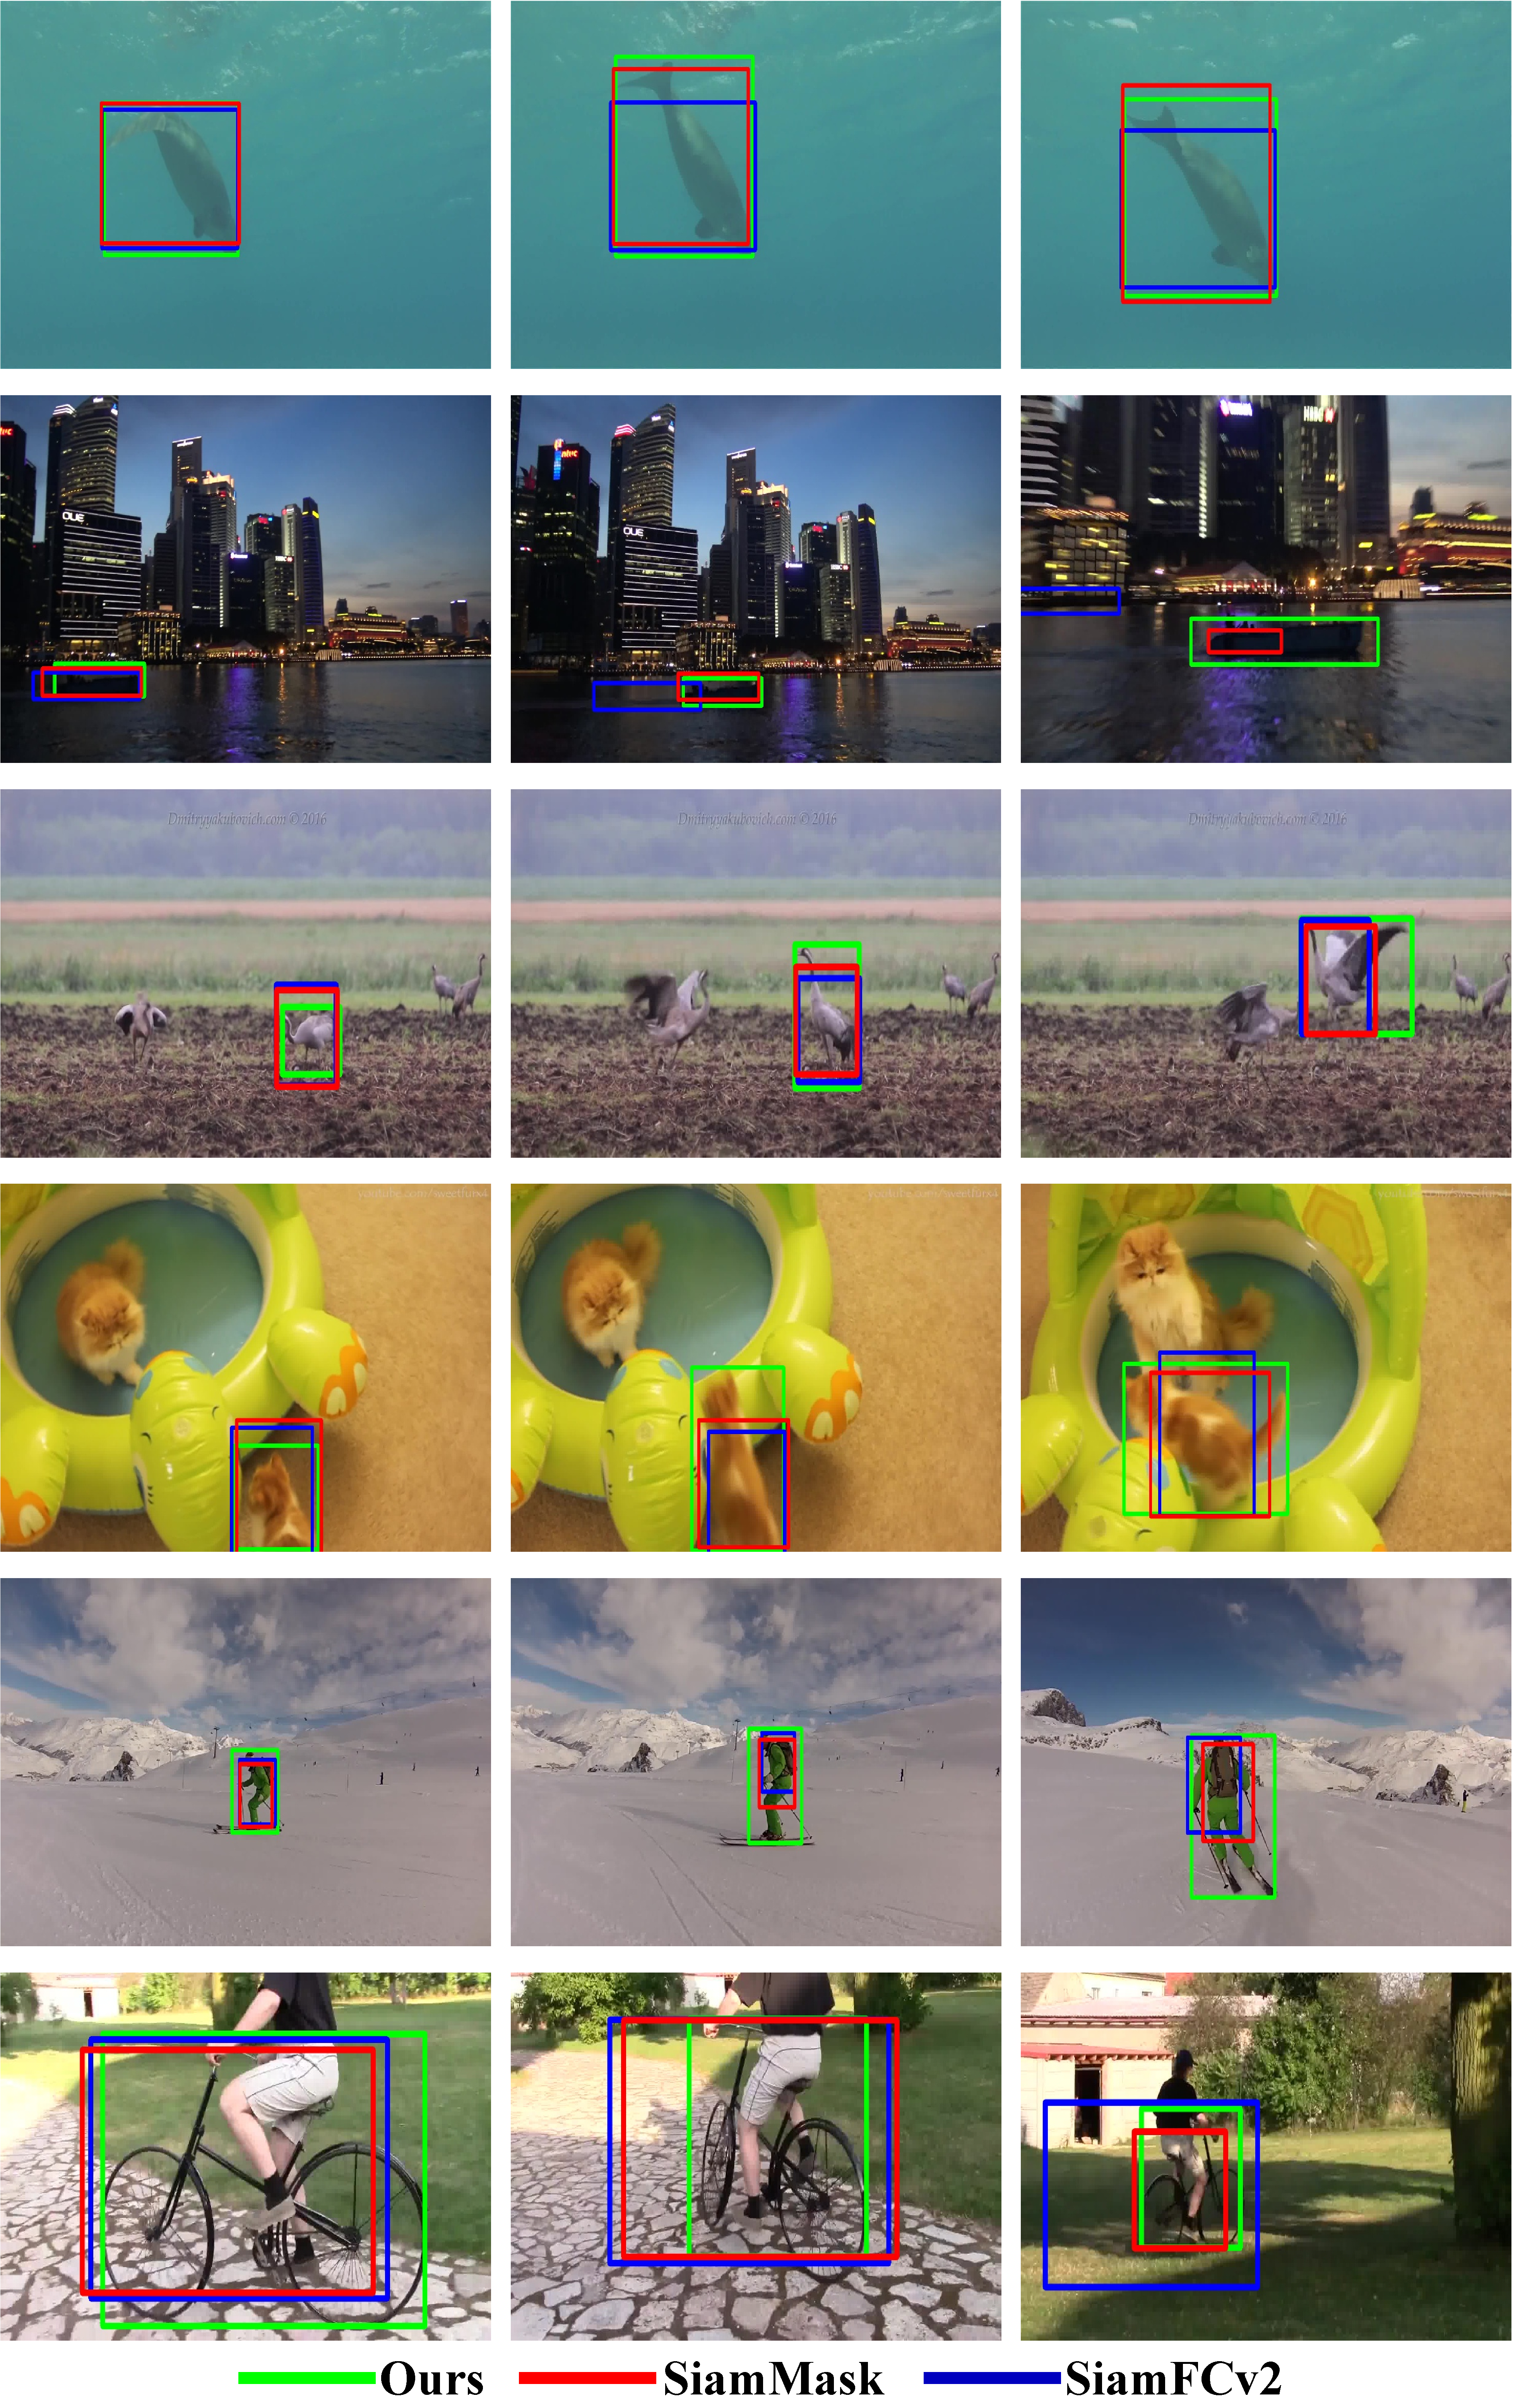
\includegraphics[width=1.0\textwidth]{Img/globally/visulization.pdf}
    \caption{我们的方法与最先进的跟踪器SiamMask \cite{Wang2018SiamMask} 和SiamFCv2\cite{SiamFC} 的比较。示例帧来自GOT-10k \cite{GOT-10k} 测试集中。
    % Our approach performs better compared to existing approaches.
    }
    \label{fig:visulization}
\end{figure}

但是,本地搜索机制有一些缺点。
首先,如果由于挑战性的照明变化,运动模糊等而导致先前帧中目标位置的预测偏离了预期,则可能会导致不可逆的累积误差,因为当前帧中生成的搜索区域可能会无法覆盖导致后续帧完全失败的目标。
其次,基于本地机制的跟踪器很难满足长期跟踪的需求 \cite{kalal2011tracking, hong2015multi}.
在长期情况下,目标经常重新进入并重新出现屏幕。
由于当目标离开并重新进入屏幕时跟踪器无法设置正确的搜索区域,因此由于错误的搜索区域而没有覆盖目标,跟踪器通常无法检索目标。

受更快的RCNN的两阶段检测范例 \cite{ren2015faster}的启发,我们提出了一种基于全局感知机制的孪生跟踪器。
在跟踪过程中,我们的跟踪器始终能够感知整个图像中的目标。
因此,即使跟踪器由于具有挑战性的目标外观变化而犯了一个错误,一旦目标的外观恢复正常,仍然可以及时检索目标。尤其是在长期视野外消失的情况下,当目标离开屏幕时跟踪器无法在完整图像中找到目标,而当目标从任何位置重新进入屏幕时,我们的跟踪器可以继续工作。

除了上述全局空间感知机制外,我们还提出了一种时间运动模型来减轻干扰因素的干扰。众所周知,基于暹罗的跟踪框架有时会受到干扰因素的困扰,因为端到端训练有素的暹罗匹配网络很难很好地区分看起来非常相似的对象。与简单设计的手工策略 \cite{SiamFC, SiamRPN}不同,我们提出的基于CNN的运动模型经过端到端训练,可以使用其历史轨迹信息和当前目标外观信息来预测目标当前位置分布。
具体来说,运动模式是在训练阶段从轨迹数据集自动学习的,而不是手工制作的特征或规则 \cite{iswanto2017visual};在测试阶段,我们可以使用任意数量的历史帧的位置信息,而不仅仅是先前的帧进行预测。

这种全球时空感知机制的另一个优势是,它使用 RoI Align \cite{He2018MaskR} 操作使跟踪器能够利用更深的网络进行特征学习,这对于流行的基于本地机制的SiamFC \cite{SiamFC} 和SiamRPN \cite{SiamRPN} 跟踪器,因为其网络结构中的填充将破坏严格的转换不变性 \cite{SiamRPN++}. 具体来说,将跟踪器中的整个模板图像和搜索图像发送到相同的主干网络以提取特征,然后根据初始帧的基本情况使用RoI Align操作从模板特征中获取对象特征。通过通道使对象特征和搜索图像特征互相关以获得融合特征图,该融合特征图被发送到后续的跟踪模块。由于此新解决方案对平移不变性没有任何限制,因此我们可以使用功能强大的ResNet \cite{he2016deep} 作为骨干网络来准确地建模前景对象与背景杂波之间的区别。

综上所述,本文做出以下三个主要贡献。
\begin{itemize}
\item 基于全局感知机制,我们引入了一个两步跟踪管道,该管道使用非常深的网络来减少累积误差并提高鲁棒性。
\item 提出了一种新颖的统一的端到端卷积神经网络的轨迹预测结构,利用历史轨迹信息和当前帧的出现信息来预测目标位置分布。
\item 我们在 GOT-10k \cite{GOT-10k} 和UAV20L \cite{mueller2016benchmark} 长期跟踪数据库上优秀的性能证明了我们提出的基于全球时空知觉的跟踪系统(GSTP)的有效性。
\end{itemize}

\section{拟议的算法}
\label{sec:method}

\iffalse
\begin{figure}[t]
    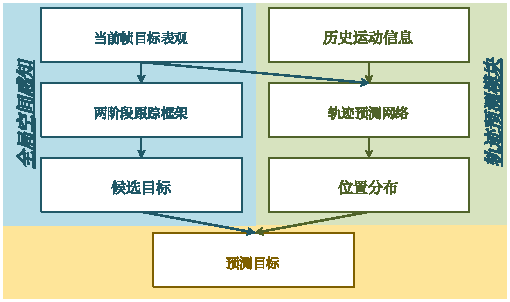
\includegraphics{images/Arch7.pdf}
    \caption{我们基于全球时空感知(GSTP)的跟踪系统的架构。}
    \label{fig:arch}
\end{figure}
\fi

\iffalse
\begin{figure*}
    \centering
    \includegraphics[width=12cm]{images/NetworkStructure1.pdf}
    \caption{The proposed tracking framework.}
    \label{fig:network}
\end{figure*}
\fi

\iffalse
\begin{figure*}
    \centering
    \includegraphics[width=12cm]{images/MotionModel.pdf}
    \caption{The effect of the motion model. SiamRCNN detects the real target (in green box) and the distractor (in red box). The motion model predicts the position distribution measuring the likelihood that the target is located at each spatial location. The motion model eliminates the distractor and preserves the real target.}
    \label{fig:motion_model}
\end{figure*}
\fi

我们的方法探索了一个关键思想,即将视觉对象跟踪任务分解为首先提取候选目标,然后使用运动模型消除干扰因素,从而可以解决该任务。
通过采用这种范例,我们可以通过设计更精确的跟踪组件和更健壮的运动模型来获得更好的性能,尤其是在长期情况下。

%要解决由本地搜索引起的累积错误,
具体而言,我们提出了全球时空感知跟踪系统,这意味着:(1)我们使用整个图像而不是小的图像块作为跟踪器的输入,以为其提供全局空间信息。 (2)为了更好地感知全局空间信息,我们提出了一个两阶段跟踪组件,该组件能够检测在视觉上类似于地面真实目标的候选目标。 (3)为了感知时间信息,我们提出了一种运动模型,该模型能够通过预测位置分布以获得最终的跟踪结果来排除干扰物。

\iffalse
Most state-of-the-art trackers adopt a one-stage framework, which performs classification and bounding box regression only once based on features obtained by cross-correlation.
In the field of object detection, the performance of two-stage detectors is usually better than that of one-stage detectors.
Inspired by this, we design our tracker as a two-stage network.
The RPN stage rapidly filters out most background samples, and the RoI head adopts a fixed foreground-to-background ratio to maintain a manageable balance between foreground and background.
In addition, two steps of regressions achieve accurate localization even for objects with extreme shapes.
\fi

\subsection{跟踪组件}

我们基于流行的对象检测架构来构建跟踪组件 --- faster RCNN \cite{ren2015faster}。尽管本文中并未首次提出使用对象检测模块和基于暹罗的特征提取器进行对象跟踪,但我们的跟踪器相对于相关跟踪算法 \cite{SiamRPN, Wang2018SiamMask, danelljan2019atom, voigtlaender2019siam}具有优势。与SiamRPN \cite{SiamRPN}的输入始终是目标位于中心的图像块相比,我们跟踪组件的输入是整个图像,这意味着目标可能出现在任何空间位置。这防止了网络学习偏向中心位置,从而打破了网络体系结构的空间不变性约束 \cite{SiamRPN++} 。结果,非常深的网络(例如ResNet50 \cite{he2016deep})可以用作跟踪组件的特征提取器。有关空间不变性限制和中心偏差的详细说明,请参考 \cite{SiamRPN++}。
%because the input of the network is the entire image, instead of the image patch centered on the target, the target will appear in any poisition in the image, so we do not need the network has strict spatial invariance restriction \cite{SiamRPN++}, so we can use a deeper feature extractor, i.e., resnet50. 
与 SiamRPN \cite{SiamRPN} 和 SiamMask \cite{Wang2018SiamMask} 相比,我们使用两阶段体系结构。第二阶段(RoI head \cite{ren2015faster})可以更有效地区分前景和背景。
与SiamMask \cite{Wang2018SiamMask} 和ATOM \cite{danelljan2019atom}相比,我们的跟踪器可以在整个图像中搜索目标,从而可以在跟踪模块出错后在空间上及时检索目标。
与骨架和RPN被冻结的Siam R-CNN \cite{voigtlaender2019siam}相比,我们的跟踪器在RPN之前会生成目标特定的功能,并且可以端到端地训练整个网络。在对象跟踪中,目标可能是一个视频中的前景而另一个视频中的背景。因此,由我们的RPN生成的候选者可以更好地满足一般对象跟踪的要求。
%(The backbone and RPN are frozen and only the redetection head (after concatenation) is trained for tracking) they fixed the parameters in the backbone and the RPN. Only the second stage is used for target spercific tracking, which is not good for "generatic" object tracking: because some objects are foreground in some cases and background in others. Instead, our tracker use the correlation before RPN, the "target" which is good for general object tracking. The architecture of our tracking component is described as follows:

%The first component of our tracking framework (i.e., SiamRCNN) is a two-stage tracker (Fig. \ref{fig:siamrcnn}) used to detect object regions that are visually similar to the given first-frame template object.
%Specifically, the tracking component consists of four modules: (1) feature extraction module, (2) feature fusion module, (3) RPN head module, and (4) RoI head module.

%The transplant from a detection task to a tracking task using faster RCNN is straightforward and easy to implement.
%, which is another advantage of our tracking module. 
为了描述我们的跟踪组件,我们首先简要回顾一下更快的RCNN。它包括一个特征提取器,其后是两个检测阶段:RPN头和RoI头。
特征提取器 $\phi_{1}$ 是ResNet50的变体。第一阶段使用区域提议网络(RPN)在主干层的最后一个特征图上滑动,并预测是否存在对象,并预测这些对象的边界框。通过执行RoI Align \cite{He2018MaskR} 以从该提议的区域提取深层特征,对RPN建议的每个区域运行第二阶段(即 RoI head)。
使用分类层将每个RoI(感兴趣区域)分类为特定类别,并使用回归层对边界框进行细化。
请参阅 \cite{ren2015faster} 了解更多详细信息。

对于对象跟踪任务,特征提取器 $\phi_{1}$有两个输入:模板图像 $z$ 和搜索图像 $x$。根据暹罗架构的设计,两个输入共享相同的网络参数以提取特征。
在生成模板特征 $f_{z} = \phi_{1}(z)$ 和搜索特征 $f_{x} = \phi_{1}(x)$之后,我们裁剪了对象特征 $f_{obj} \in \mathbb{R}^{1024 \times 7 \times 7}$ 由RoI Align操作 \cite{He2018MaskR} 根据目标的实际情况从模板特征中获取:
\begin{equation}
    f_{obj} = \mathcal{R}(b_{obj}, f_{z}),
\end{equation}
其中 $\mathcal{R}$ 表示RoI Align运算符,而 $b_{obj}$ 是目标的地面真值边界框。
接下来,通过深度互相关 \cite{SiamRPN++} 合并搜索功能和对象功能:
\begin{equation}
    f_{corr} = f_{obj} * f_{x},
\end{equation}
其中 $f_{corr}$ 是融合特征和 $*$ 是深度方向互相关算子。
%The use of RPN (region proposal network) is ...
然后将 $f_{corr}$ 发送到RPN头以生成候选 $B=\{b^{i}_{roi}\}^{i=1:N}$.
\iffalse
There are two inputs to the feature extraction module: the template image $z$ and the search image $x$. According to the design of the siamese architecture, the two inputs share the same network parameters to extract features.
The network structure of the feature extraction module is a variant of ResNet50, which is pretrained on the 1000-class ImageNet classification set. Features of the input images are extracted from the final convolution layer of the 4-th stage. The obtained template features $f_{z} = \phi(z)$ and search features $f_{x} = \phi(x)$ with channel dimension 1024 and stride 16 are sent to the subsequent feature fusion module.

In the feature fusion module, object features $f_{obj}$ are obtained by the RoI Align operation from the template features according to the ground truth of the target. The search features and the object features are merged via the depth-wise cross-correlation:
\begin{equation}
    f_{obj} = \mathcal{R}(b_{obj}, f_{z})
\end{equation}
where $\mathcal{R}$ represents the RoIAlign, $\odot$ represents the element-wise multiplication, $b$ represents an RoI in candidate proposals and $\mathcal{X}$ represents the fused feature of $b$.
\begin{equation}
    f_{corr} = f_{obj} * f_{x}.
\end{equation}
Two 1 $\times$ 1 convolutions with channel dimension 1024 are added on top of the correlation layer to obtain the fusion feature.

The RPN head includes two sibling 1 $\times$ 1 convolutional layers -- a classification layer with channel dimension 2$k$, and a regression layer with channel dimension 4$k$, where $k$ is the number of maximum possible proposals for each location. The RPN head takes the fusion feature as input and simultaneously regress region bounds and objectness scores for each anchor.
\fi
%The RoI head is run for each region proposed by the RPN by performing RoI Align \cite{He2018MaskR} to extract deep features from this proposed region.
在第二阶段,对融合特征 $f_{corr}$执行RoI Align操作,为每个RoI生成一个小特征图,其通道尺寸为2048,固定空间范围为 7 $\times$ 7:
\begin{equation}
    f_{roi}^{i} = \mathcal{R}(b_{roi}^{i}, f_{corr}),
\end{equation}
其中 $b_{roi}^{i}$ 是候选区域 $i$的边界框。
最后,每个RoI被分类为前景/背景。在测试期间,我们选择排名靠前的 $K$ 的RoI作为候选目标,这些目标将在运动模型中进行后处理。

\iffalse
The RoI Aligned features are fed into the global average pooling layer followed by two sibling output layers: one that produces softmax probability estimates over two classes (foreground or background) and another layer that outputs four real-valued numbers for the foreground class. These four values encode the refined bounding-box position for the RoI.
The loss of SiamRCNN is:
$$Loss = L_{cls}^{rpn} + L_{cls}^{roi} + \lambda (L_{reg}^{rpn}+L_{reg}^{roi}),$$
where $\lambda$ is hyper-parameter to balance the classification loss and the regression loss. $L_{cls}^{*}$
is the cross entropy loss and $L_{reg}^{*}$ is the standard smooth $L1$ loss for regression.
\fi

\iffalse
\begin{figure*}
    \centering
    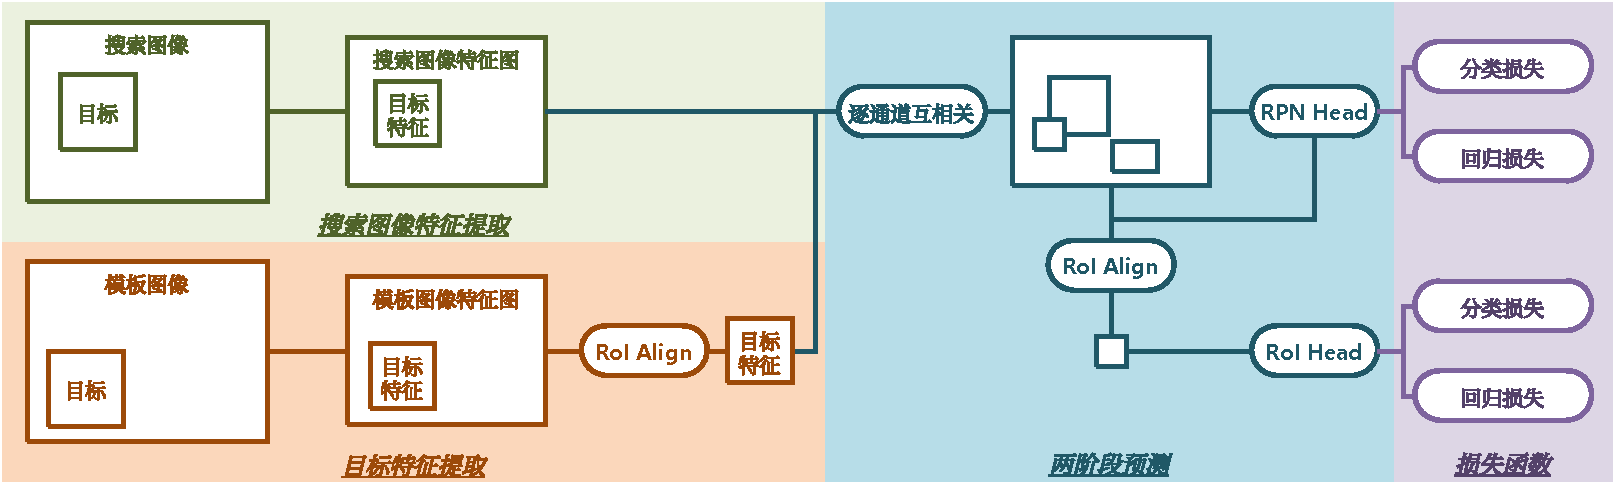
\includegraphics[width=17cm]{images/SiamRCNN.pdf}
    \caption{Architecture of SiamRCNN.}
    \label{fig:siamrcnn}
\end{figure*}
\fi

\subsection{运动模型} 使用我们的跟踪组件检测到与给定的第一帧模板对象在视觉上相似的对象区域后,我们使用运动模型消除干扰因素并获得最终的跟踪结果。
通过使用历史轨迹信息和当前帧的外观信息学习目标位置分布,运动模型以端到端的方式工作。
然后,它根据位置分布重新评估候选目标,该位置分布是一个二维热图,用于测量目标位于每个空间位置的可能性。

令 $H_{t}^{k} = \{h_{t-i}\}_{i=1:k}$ 表示历史轨迹信息,其中 $t$ 是当前帧的索引,$k$ 是历史长度,并且 $h_{j} = \{x_{j}, y_{j}\}$ 是一个二维坐标,表示目标在帧 $j$中的位置。
受姿态估计任务的启发,我们将 $h_{j}$ 表示为二维热图 $m_{j} \in \mathbb R^{h \times w}$ ,其中二维高斯定点位于目标位置 $(x_{j}, y_{j})$。
为了对时间信息进行建模,根据时间顺序将生成的 $k$ 热图进行连接,以获得通道张量 $\mathcal{M} \in \mathbb{R}^{k \times h \times w}$ 维度 $k$:
\begin{equation}
    \mathcal{M}_{t}^{k} = \mathcal{C}(m_{t-k}, m_{t-k+1}, ..., m_{t-1}),
\end{equation}
其中 $\mathcal{C}(\cdot)$ 是串联操作。

我们的运动模型不是仅仅利用历史轨迹信息进行预测,但也考虑当前帧的出现信息。
为此,将当前帧 $\mathcal{I} \in \mathbb{R}^{3 \times h \times w}$ 的RGB图像与轨迹张量连接起来,以获得增强的轨迹张量 $\mathcal{N} \in \mathbb{R}^{(3+k) \times h \times w}$ ,通道尺寸为 $(3+k)$:
\begin{equation}
    \mathcal{N}_{t}^{k} = \mathcal{C}(\mathcal{I}_{t}, \mathcal{M}_{t}^{k}).
\end{equation}
假设 $\phi_{2}$ 是运动模型,它是一个CNN网络,则 $\phi_{2}$ 的输出计算如下:
\begin{equation}
    \mathcal{O}_{t}^{k} = \phi_{2}(\mathcal{N}_{t}^{k}),
\end{equation}
其中 $\mathcal{O}_{t}^{k} \in \mathbb{R}^{h \times w}$ 是二维热图,它反映了目标在 $t$帧中的位置分布。

我们的运动模型 $\phi_{2}$ 的网络与姿势估计网络HRNet \cite{sun2019deep}相同。
\iffalse
The main reason why the pose estimation network can be used to design the motion model is that the output of the pose estimation network is the position distribution of joint points, and the output of the motion model is the position distribution of the target. This means that there is a great deal of commonality between the two tasks. In order to use HRNet for trajectory estimation, we need to change the input and output of HRNet and keep the network structure unchanged.

During tracking the $i$-th frame, we utilize the position information of the previous $K$ frames as the input to the network.
Specifically, for a historical frame, a heat map is generated by applying 2D Gaussian with stand deviation of 3 pixels centered on the target position in that frame.
The generated $K$ heatmaps are concatenated according to the time order to obtain the \textbf{trajectory tensor} with channel dimension $K$.
Our motion model not only utilizes the historical trajectory information for prediction, but also considers the appearance information of the current frame.
To achieve this, the RGB image of the current frame and the trajectory tensor are concatenated to obtain the tensor with channel dimension $(3+K)$. This tensor is sent to the network, and the output of the network is a heatmap reflecting the position distribution of the target in the current frame. The loss function, defined as the mean squared error, is applied for comparing the predicted heatmap and the groundtruth heatmap. The groundtruth heatmap is generated by applying 2D Gaussian with standard deviation of 3 pixels centered on the target position in the current frame. The network structure of our motion model is the same as HRNet. 
\fi
这里提供简要说明。 HRNet的第一阶段是高分辨率子网。然后,从高到低分辨率的子网一一添加,以形成更多的阶段。多分辨率子网并联连接。通过在整个过程中一遍又一遍地在并行多分辨率子网中交换信息来进行重复的多尺度融合。我们估计HRNet输出的高分辨率表示上的位置分布。有关网络结构的详细信息,请参考 \cite{sun2019deep}。

\section{实验}
\label{sec:experiments}
\iffalse
\begin{figure}[htb]
    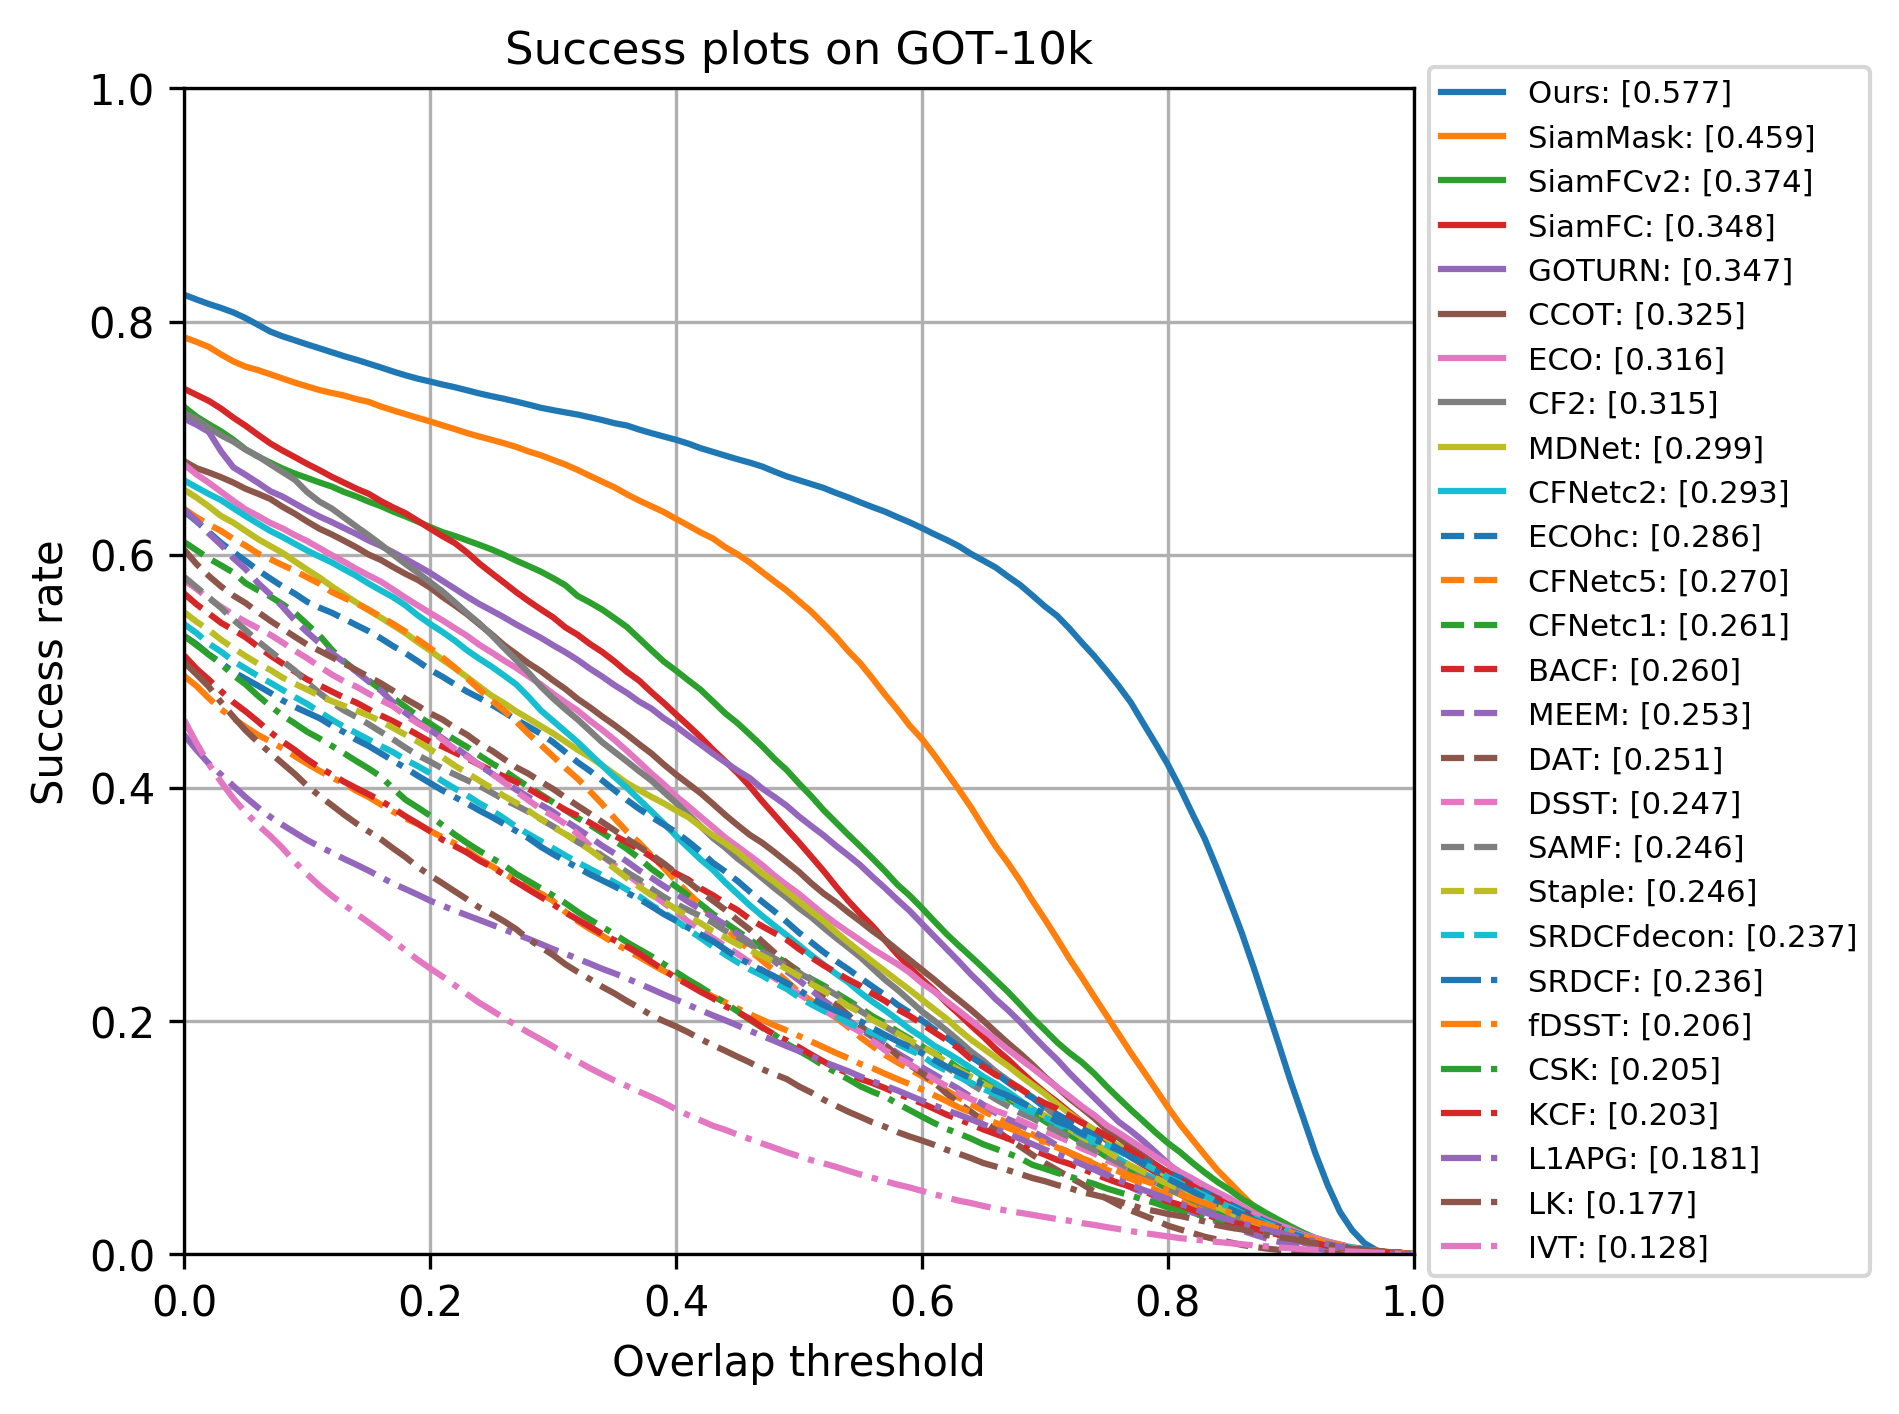
\includegraphics[width=8.6cm]{images/success_plot.png}
    \caption{Overall performance on GOT-10k, ranked by their average overlap (AO) scores.
}
    \label{fig:ao}
\end{figure}
\fi

\subsection{实施细节}
我们的跟踪组件在GOT-10k \cite{GOT-10k} 训练集中进行了训练。它包含超过10000个真实运动对象的视频片段和超过150万个手动标记的边界框,其中包括563类真实运动对象和87类运动模式。
我们执行多尺度训练:目标大小从 $64 \times 64$ to $256 \times 256$不等。图像大小在跟踪过程中保持不变。跟踪组件使用随机梯度下降(SGD)进行训练。我们使用 $10^{-4}$ 的权重衰减和0.9的动量。我们训练跟踪组件进行27k次迭代。学习率从 $10^{-2}$ 降至 $10^{-4}$。

运动模型也通过GOT-10k训练集进行训练。 Adam优化器 \cite{kingma2014adam} 用于培训。基本学习率设置为 $10^{-3}$,并在第170和200个时代分别降至 $10^{-4}$ 和 $10^{-5}$ 。训练过程在210个纪元内终止。

\subsection{对GOT-10k数据集的评估}
在本小节中,我们在GOT-10k \cite{GOT-10k} 数据集上评估我们的方法。
GOT-10k的评估指标包括平均重叠(AO)和成功率(SR)。 AO表示所有地面和估计边界框之间重叠的平均值,而SR表示重叠超过0.5 / 0.75的成功跟踪帧的百分比。

\textbf{对比实验}
从表 \ref{tabel:ablation}(第 $1^{st}$ 行和第 $2^{nd}$ 行)中,我们看到,通过添加RoI头,AO性能提高了11.1%。 RPN阶段可快速过滤掉大多数背景样本,并且RoI头采用固定的前景与背景比率,以在前景与背景之间保持可管理的平衡。
从表 \ref{tabel:ablation} (第 $2^{nd}$ 行和第 $3^{rd}$ 行)中,我们可以看到运动模型,AO,SR$_{0.50}$和SR$_{0.75}$ 分别增加 3.9\%,5.0\% 和 1.7\%。这是因为所提出的运动模型可以有效地预测目标的位置分布,从而有效地避免了干扰因素的不利影响。

\textbf{总体效果}
我们在GOT-10k测试装置上将我们提出的方法与8个跟踪器(包括最新技术)进行了比较。
%To reflect the generalization ability, all deep learning based trackers are trained using the GOT-10k training set.
\begin{table}
\centering
\caption{我们的算法在GOT-10k测试集上具有不同组件的性能。}
\begin{tabular}{c c c c c}
\bottomrule
ROI head & Motion model & $AO$ & $SR_{0.50}$ & $SR_{0.75}$ \\ 
\hline
          &           & 0.410 & 0.486 & 0.162 \\
\checkmark&           & 0.521 & 0.595 & 0.440 \\
\checkmark&\checkmark & 0.560 & 0.645 & 0.457 \\
\bottomrule
\label{tabel:ablation}
\end{tabular}
\end{table}
\begin{table}
\centering
\caption{将我们的方法的结果与GOT-10k测试集上的其他方法进行比较。跟踪器按其平均重叠(AO)分数排名。}
\begin{tabular}{l l l l}
\bottomrule
Method   &  $AO$   &  $SR_{0.50}$ & $SR_{0.75}$  \\
\hline
Ours &  $\textbf{0.560}^\textbf{1}$ & $\textbf{0.645}^\textbf{1}$  & $\textbf{0.457}^\textbf{1}$  \\
SiamMask &  0.459&  0.560 &0.205 \\
SiamFCv2 &  0.374&  0.404 &0.144 \\
SiamFC   &  0.348&  0.353 &0.098 \\
GOTURN	 &  0.347&  0.375 &0.124 \\
CCOT	 &  0.325&  0.328 &0.107 \\
ECO	     &  0.316&  0.309 &0.111 \\
CF2	     &  0.315&  0.297 &0.088 \\
MDNet	 &  0.299&  0.303 &0.099 \\
%CFNetc2	 &  0.293&  0.265 &0.087 \\
%ECOhc	 &  0.286&  0.276 &0.096 \\
\bottomrule
\end{tabular}
\label{table:got}
\end{table}
%The success plot of the evaluated trackers is shown in Fig. \ref{fig:ao}.
与列出的方法相比,我们的方法实现了0.560的出色AO(表\ref{table:got})。
%CSK is a typical DCF-based tracker, which uses a well-established theory of Circulant matrices to derive closed-form solutions for training and detection with several types of kernels. In contrast, our tracker is based on powerful CNNs. As a result, our tracker significantly outperforms CSK with a relative gain of 173.17\% in terms of AO, which suggests the excellence of the CNN framework as well as the effectiveness of GSTP.
%MDNet learns shared layers and multiple branches of domain-specific layers, where domains correspond to individual training sequences and each branch is responsible for binary classification to identify target in each domain. In contrast, our tracker learns a general similarity map by cross-correlation between the feature representations learned for the target template and the search region. Compared with MDNet, the relative improvement of the AO score is 87.29\%, which suggests that the Siamese architecture and the cross-correlation operation are more suitable for the object tracking task.
%SiamMask is one of state-of-the-art trackers. It is a Siamese tracker and takes advantage of very deep networks to extract features. SiamMask utilizes the region proposal subnetwork to predict the location of the target. 
与SiamMask \cite{Wang2018SiamMask}相比,我们的两阶段跟踪器是基于全局感知机制设计的,可以减少累积的误差。运动模型可抑制干扰因素并提高跟踪的鲁棒性。结果,我们的跟踪器在AO方面的性能要比SiamMask高22.00%,这凸显了所提出的跟踪器和运动模型的重要性。

\textbf{按属性进行的性能分析} 
\begin{table}
\centering
\caption{Performance on subsets with different attributes collected from GOT-10k validation set.}
\begin{tabular}{|c|c|c|c|c|c|c|}
\hline
\multirow{2}{*}{Att.} &
\multicolumn{2}{c|}{SiamFC} & \multicolumn{2}{c|}{SiamMask} &\multicolumn{2}{c|}{Ours} \\
\cline{2-7} & $AO$ & $SR_{0.5}$ & $AO$ & $SR_{0.5}$ & $AO$ & $SR_{0.5}$ \\
\hline
FM & 0.472 & 0.538 & 0.526 & 0.608 & 0.639 & 0.715 \\
\hline
OC & 0.411 & 0.447 & 0.494 & 0.559 & 0.585 & 0.659 \\
\hline
CU & 0.505 & 0.545 & 0.595 & 0.701 & 0.738 & 0.837 \\
\hline
LO & 0.557 & 0.655 & 0.643 & 0.779 & 0.721 & 0.807 \\
\hline
\end{tabular}
\label{table:attribute}
\end{table}
GOT-10k训练/验证数据集中的每个视频都带有多个属性,包括:可见比率,运动速度,视频长度和按图像分割。为了分析各种情况下的跟踪器性能,我们将跟踪器与两个最新的跟踪器(即 SiamFC  \cite{SiamFC} 和 SiamMask \cite{Wang2018SiamMask})在 GOT-10k 验证集上进行了比较。我们根据属性注释从验证集中收集四个子集:FM(快速运动)子集,OC(遮挡)子集,CU(按图像剪切)子集和LO(长视频)子集。
FM子集包括目标运动速度快的视频。
OC子集包括经常遮挡目标的视频。
CU子集包括视频,其中目标经常被图像边界切割。
LO子集包括验证集中最长的40个视频。
表 \ref{table:attribute} 显示了跟踪算法的不同性能特征。
在FM子集上,我们的方法在AO方面的表现优于 \cite{Wang2018SiamMask} with a relative gain of 21.48\% in terms of AO. 
%This result suggests that our motion model is capable of modeling challenging motion patterns.
在AO方面,我们的算法在OC和CU子集上的性能分别比SiamMask高18.42%和24.03%。
%This result suggests that our two-stage tracker based on ResNet50 is able to handle the appearance changes caused by heavy occlusion.
在LO子集上,与SiamMask相比,AO得分的相对提高为12.13%。结果表明,全局感知机制使我们的跟踪器可以减少跟踪长视频时的累积误差。

\subsection{对UAV20L数据集的评估}

\begin{figure}[htb]
\begin{minipage}[b]{0.5\linewidth}
  \centering
  \centerline{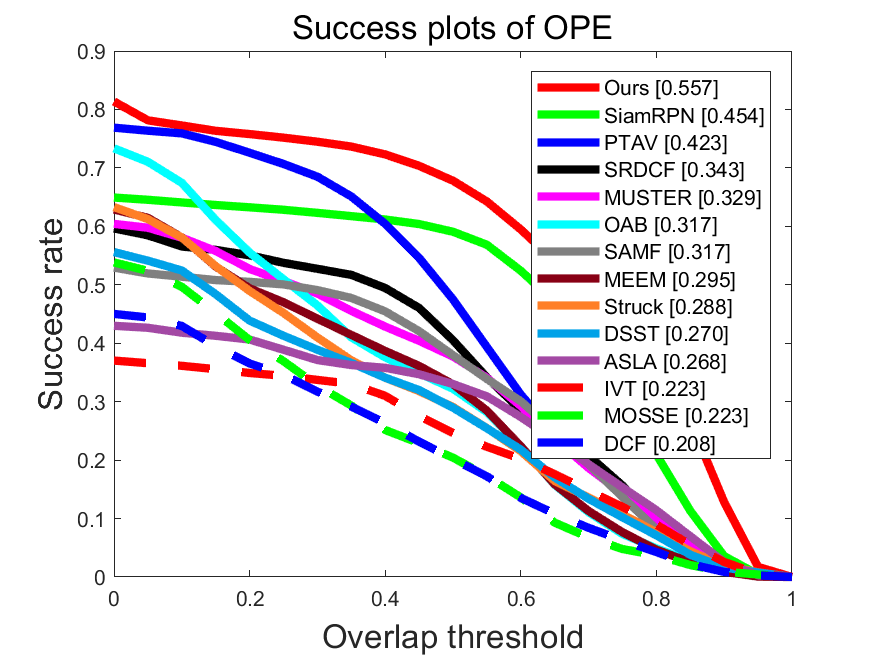
\includegraphics[width=1.0\textwidth]{Img/globally/UAV20L/quality_plot_overlap_OPE_AUC.png}}
\end{minipage}
\hfill
\begin{minipage}[b]{0.5\linewidth}
  \centering
  \centerline{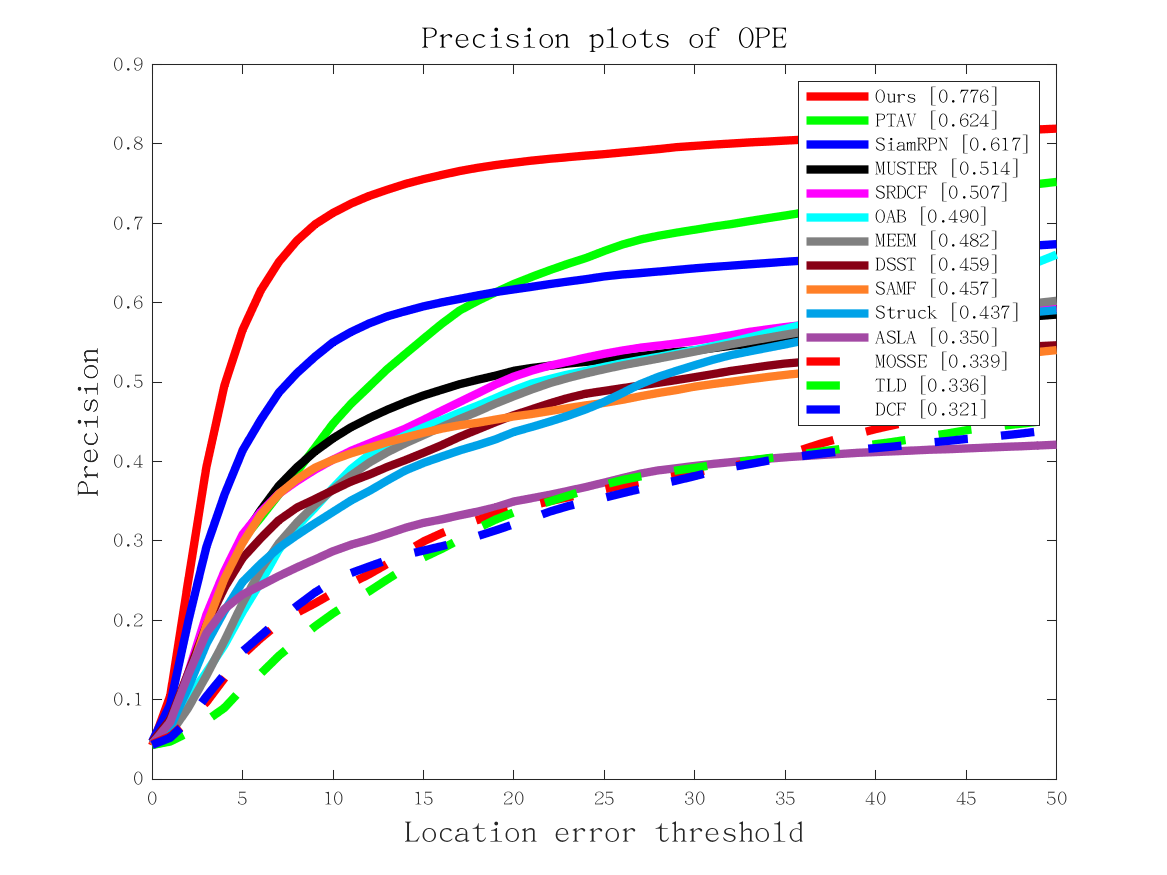
\includegraphics[width=1.0\textwidth]{Img/globally/UAV20L/quality_plot_error_OPE_threshold.png}}
\end{minipage}
%
\caption{UAV20L数据集上的成功图和精度图。}
\label{fig:uav20l}
%
\end{figure}

\iffalse
\begin{figure}[t]
\begin{center}
\subfigure[]{
	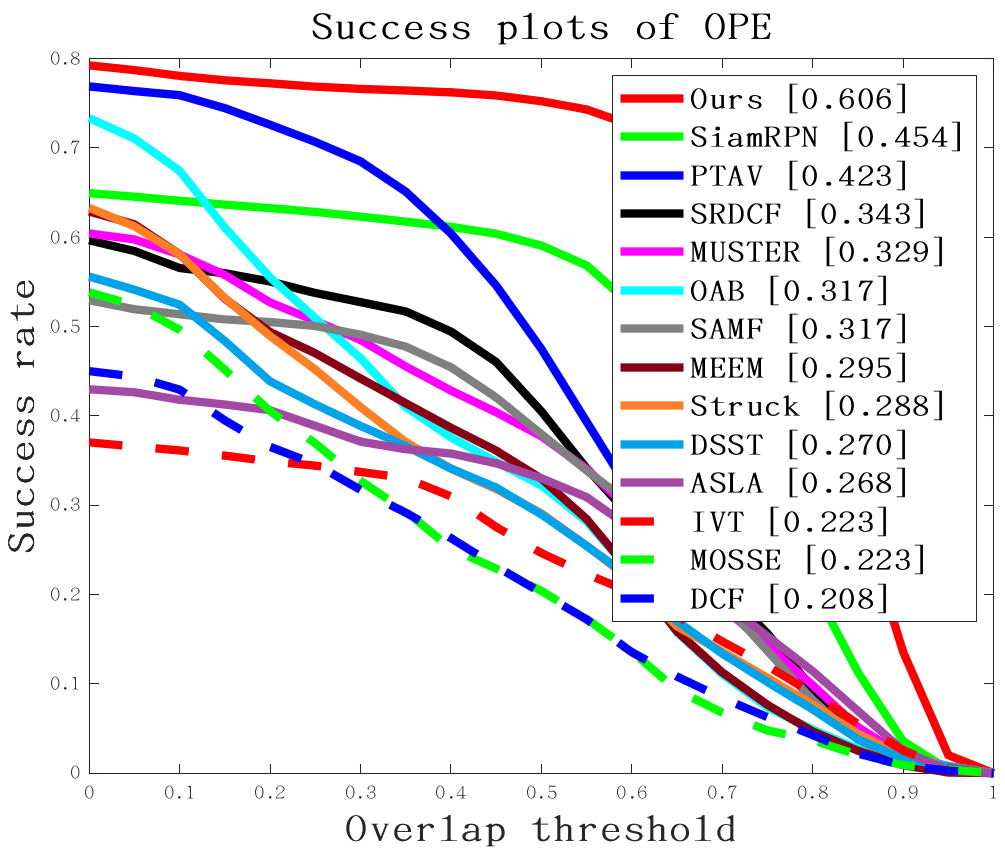
\includegraphics[width=0.47\linewidth]
	{images/UAV20L/quality_plot_overlap_OPE_AUC.png}
}
\subfigure[]{
	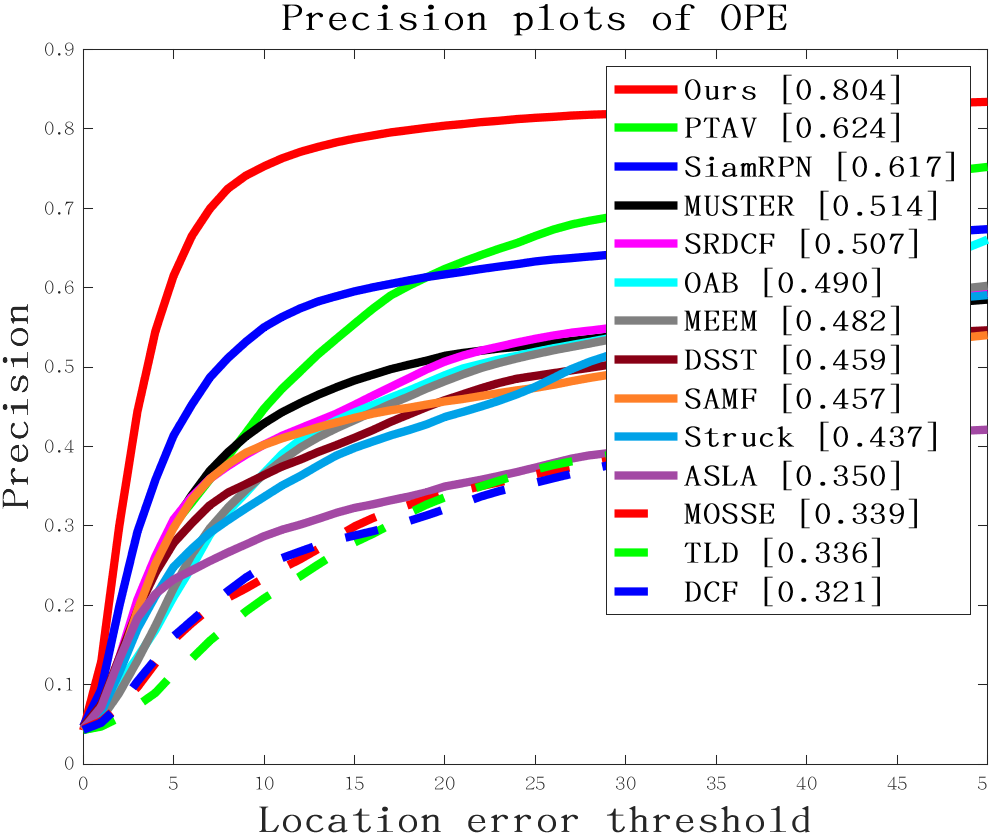
\includegraphics[width=0.47\linewidth]
	{images/UAV20L/quality_plot_error_OPE_threshold.png}
}
\end{center}
   \caption{Success and precision plots on UAV20L dataset.}
\label{fig:uav20l}
\end{figure}

\begin{figure*}
\begin{center}
\subfigure[]{
	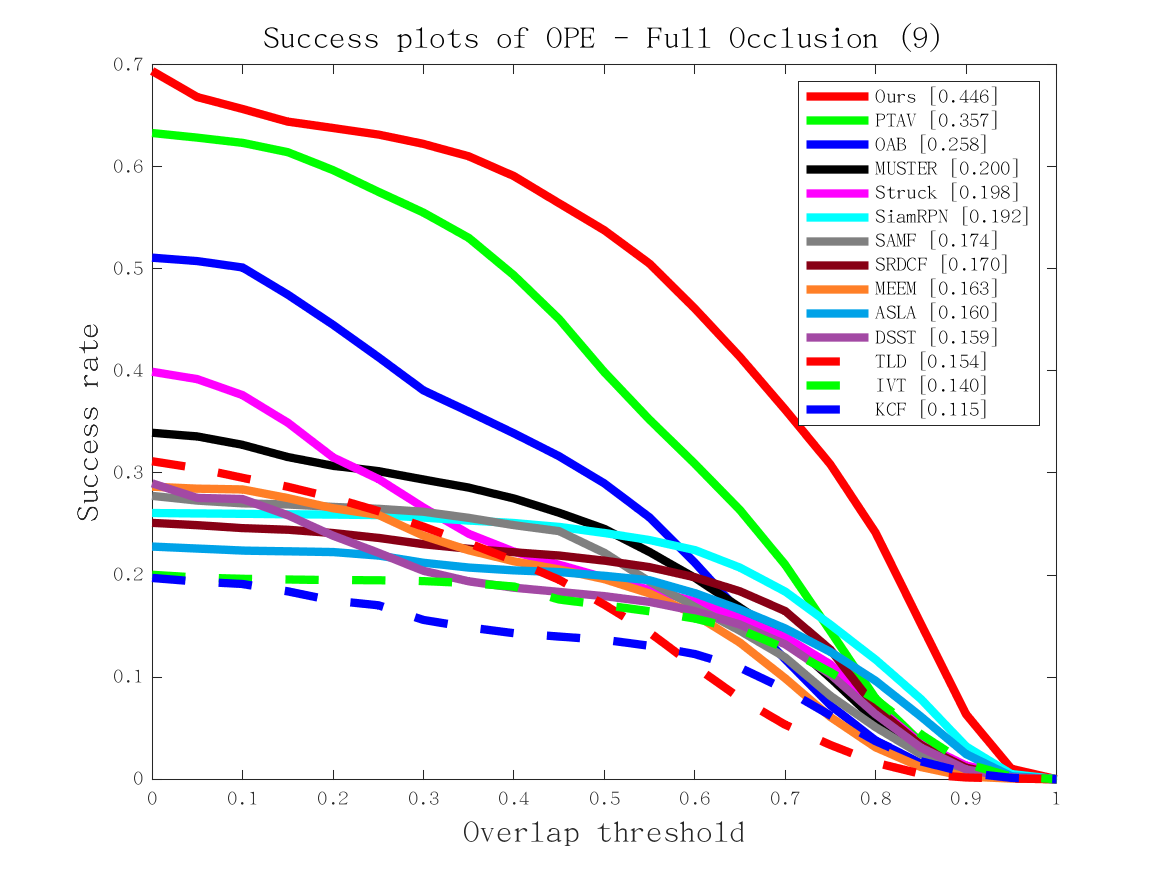
\includegraphics[width=0.234\linewidth]
	{images/UAV20L/FOC_overlap_OPE_AUC.png}
}
\subfigure[]{
	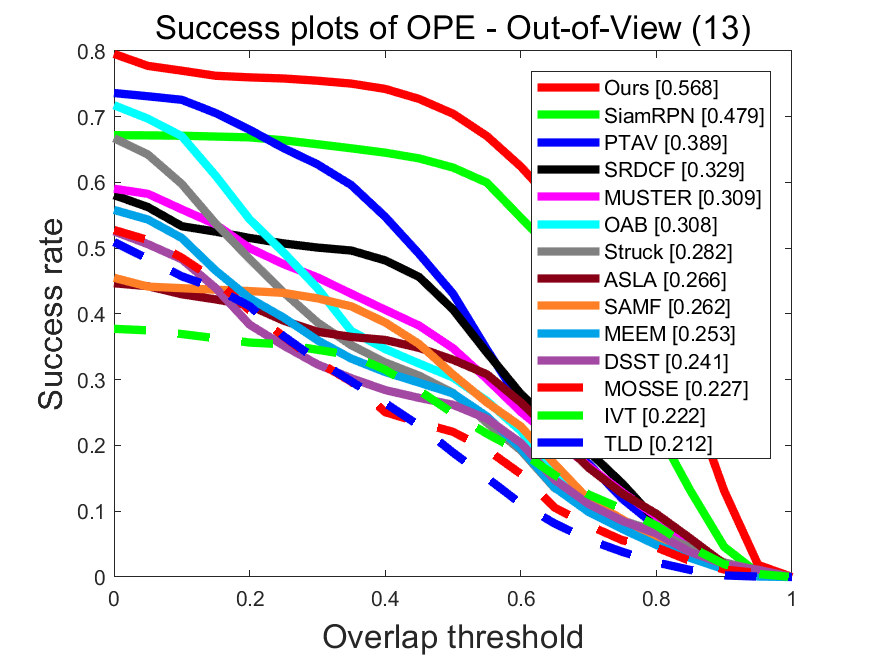
\includegraphics[width=0.234\linewidth]
	{images/UAV20L/OV_overlap_OPE_AUC.png}
}
\subfigure[]{
	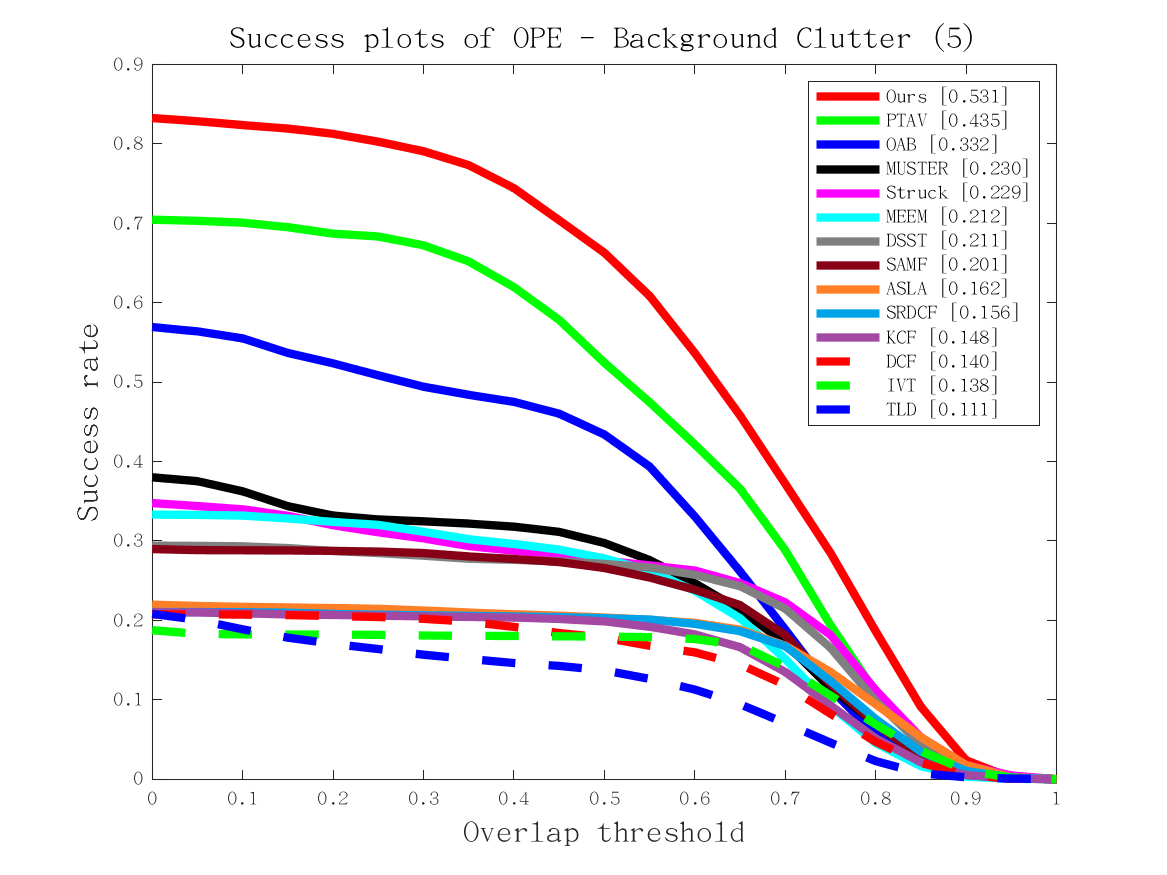
\includegraphics[width=0.234\linewidth]
	{images/UAV20L/BC_overlap_OPE_AUC.png}
}
\subfigure[]{
	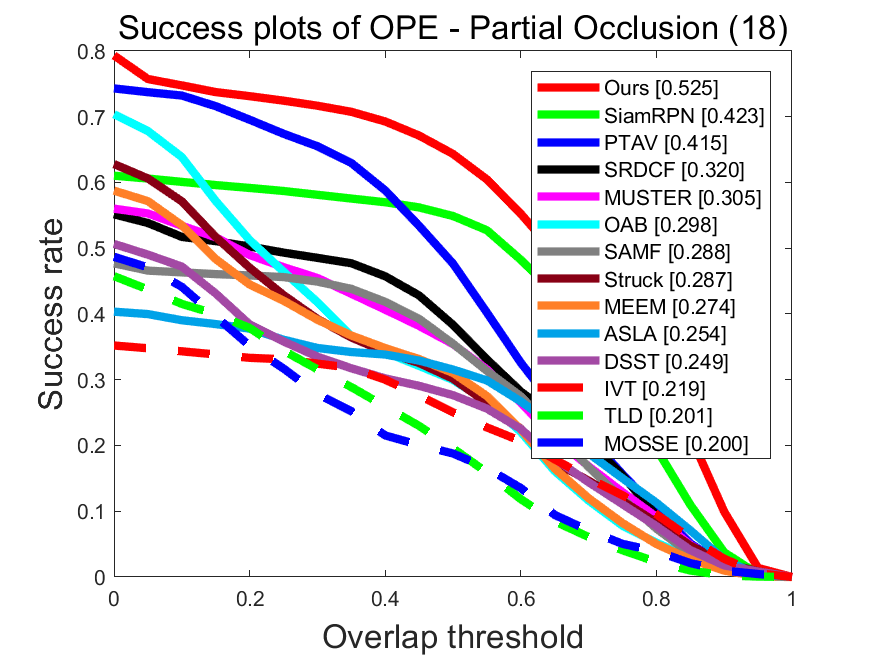
\includegraphics[width=0.234\linewidth]
	{images/UAV20L/POC_overlap_OPE_AUC.png}
}
\subfigure[]{
	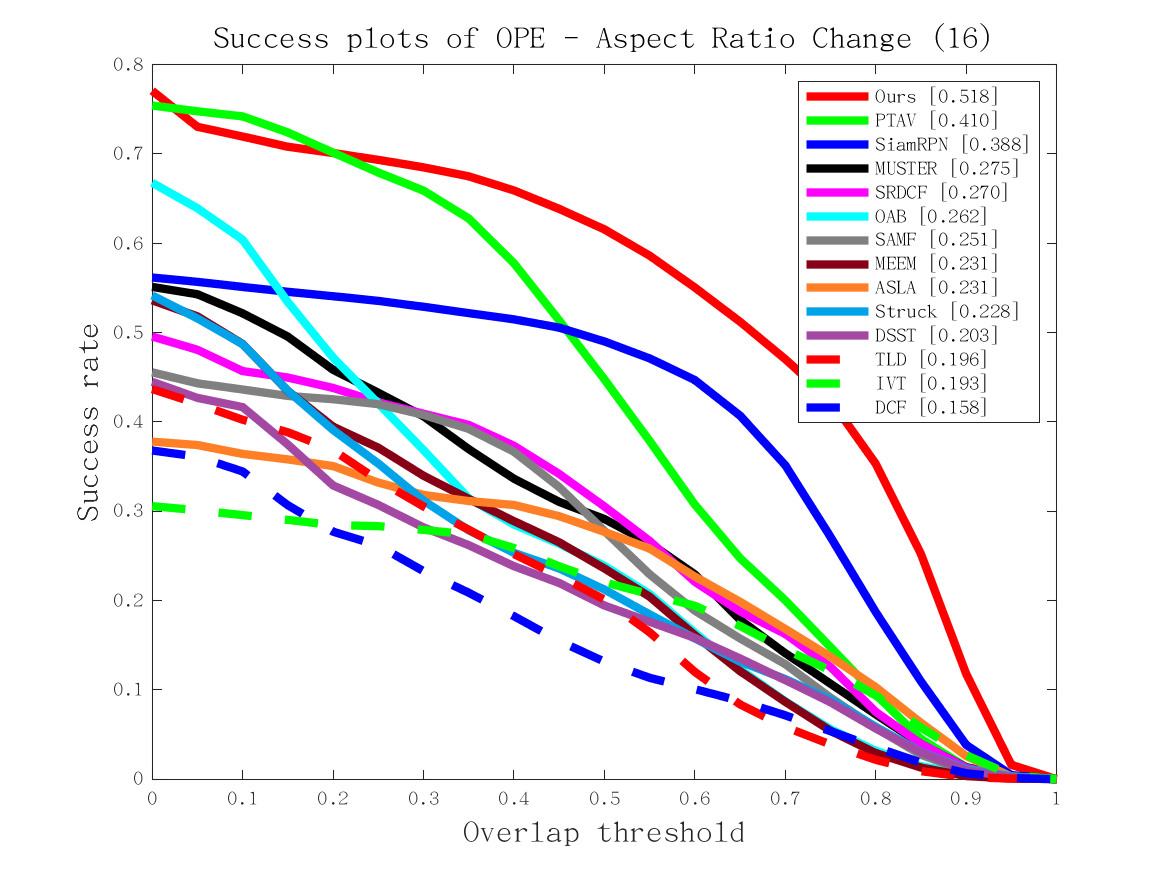
\includegraphics[width=0.234\linewidth]
	{images/UAV20L/ARC_overlap_OPE_AUC.png}
}
\subfigure[]{
	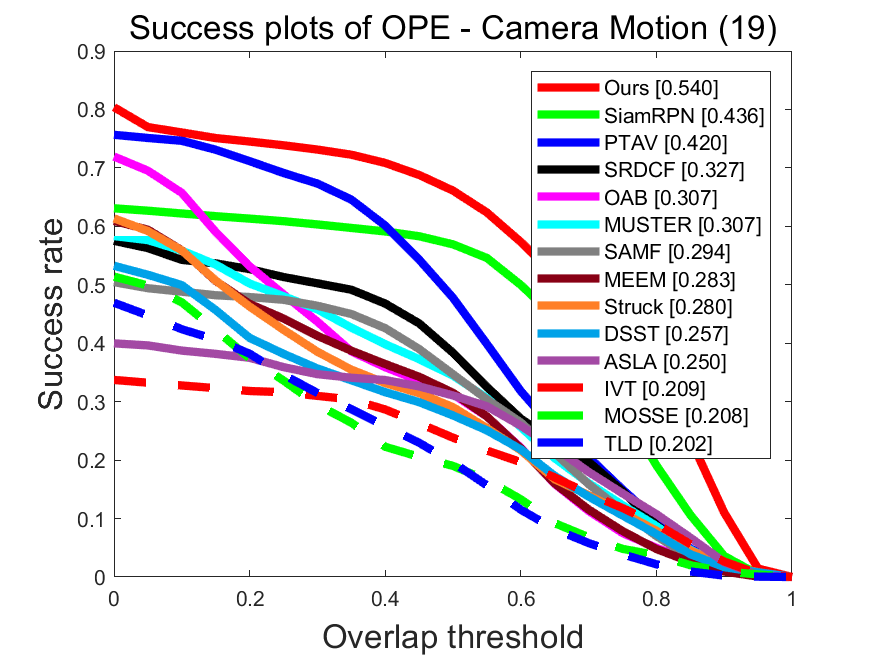
\includegraphics[width=0.234\linewidth]
	{images/UAV20L/CM_overlap_OPE_AUC.png}
}
\subfigure[]{
	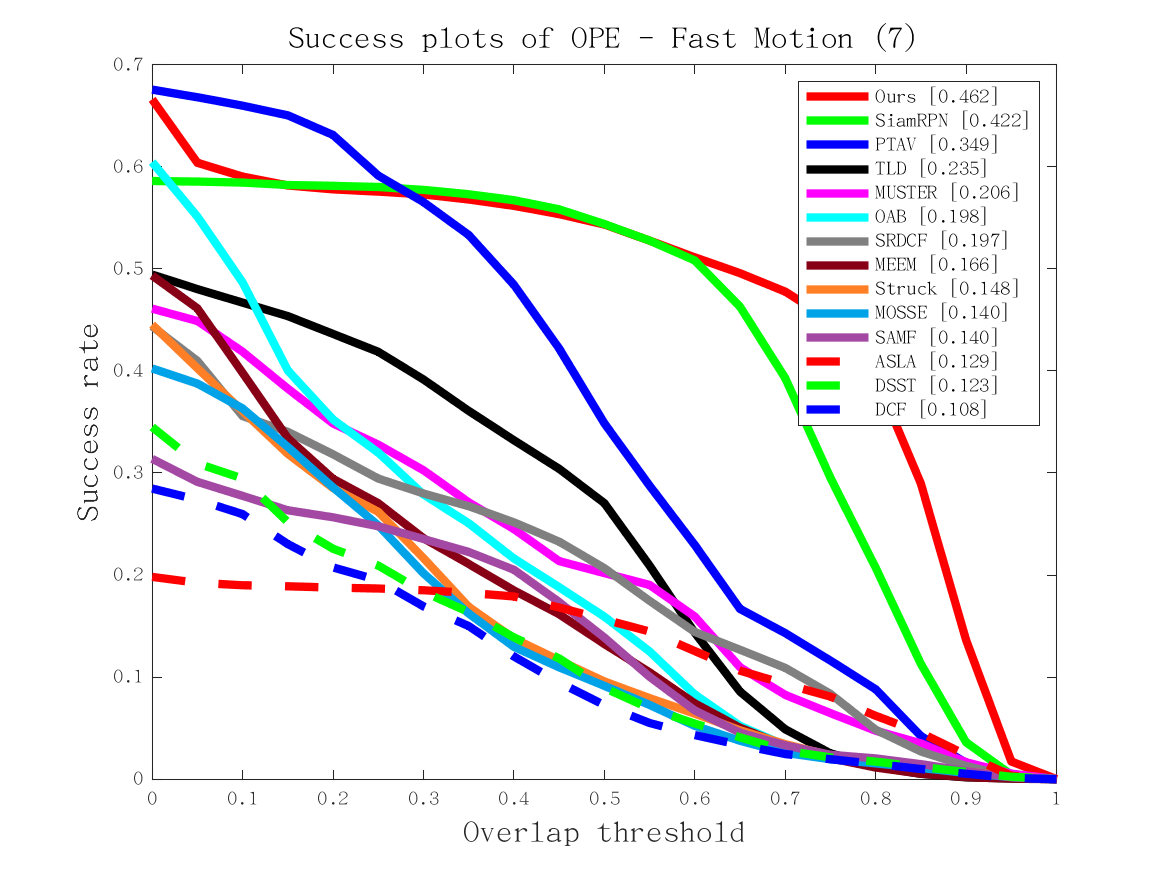
\includegraphics[width=0.234\linewidth]
	{images/UAV20L/FM_overlap_OPE_AUC.png}
}
\subfigure[]{
	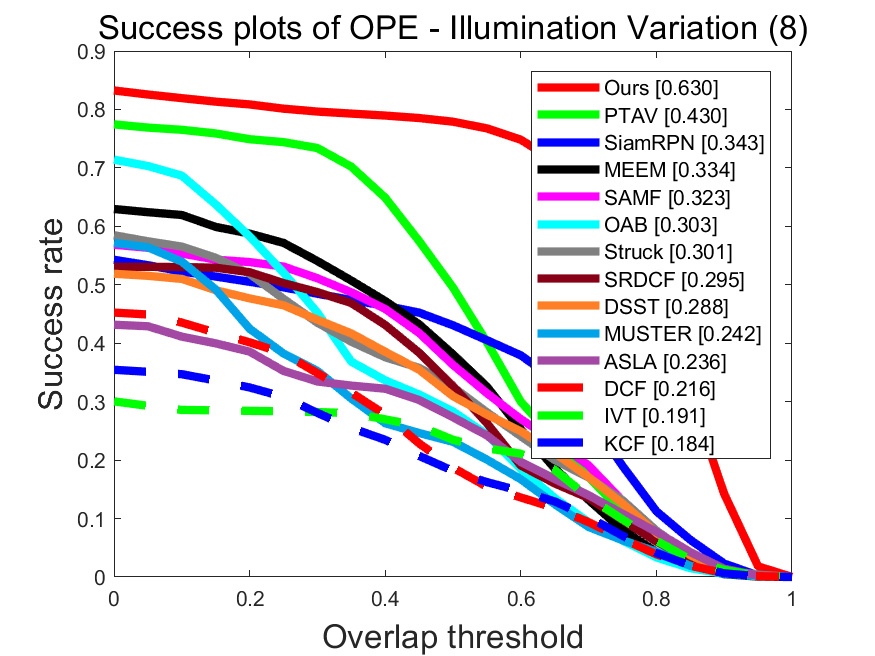
\includegraphics[width=0.234\linewidth]
	{images/UAV20L/IV_overlap_OPE_AUC.png}
}
\subfigure[]{
	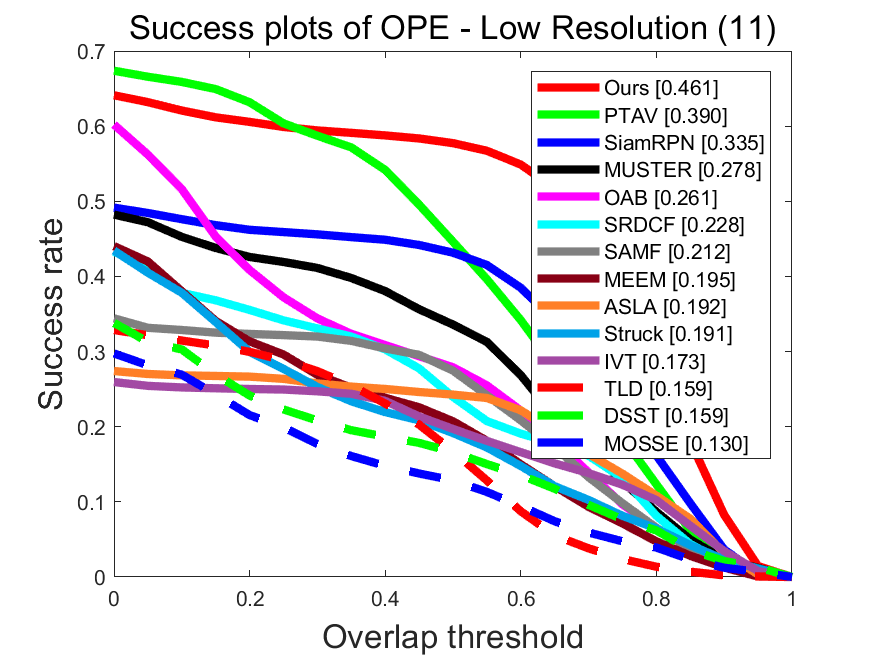
\includegraphics[width=0.234\linewidth]
	{images/UAV20L/LR_overlap_OPE_AUC.png}
}
\subfigure[]{
	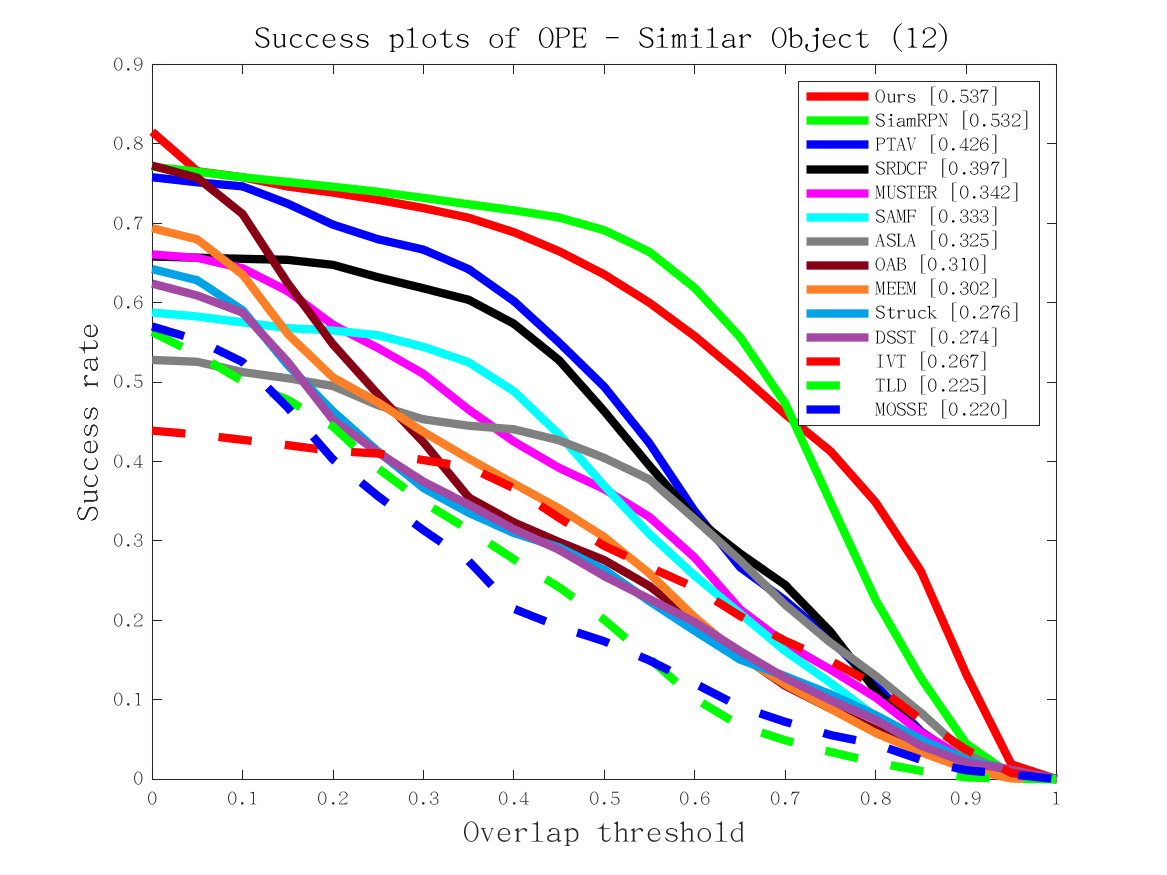
\includegraphics[width=0.234\linewidth]
	{images/UAV20L/SOB_overlap_OPE_AUC.png}
}
\subfigure[]{
	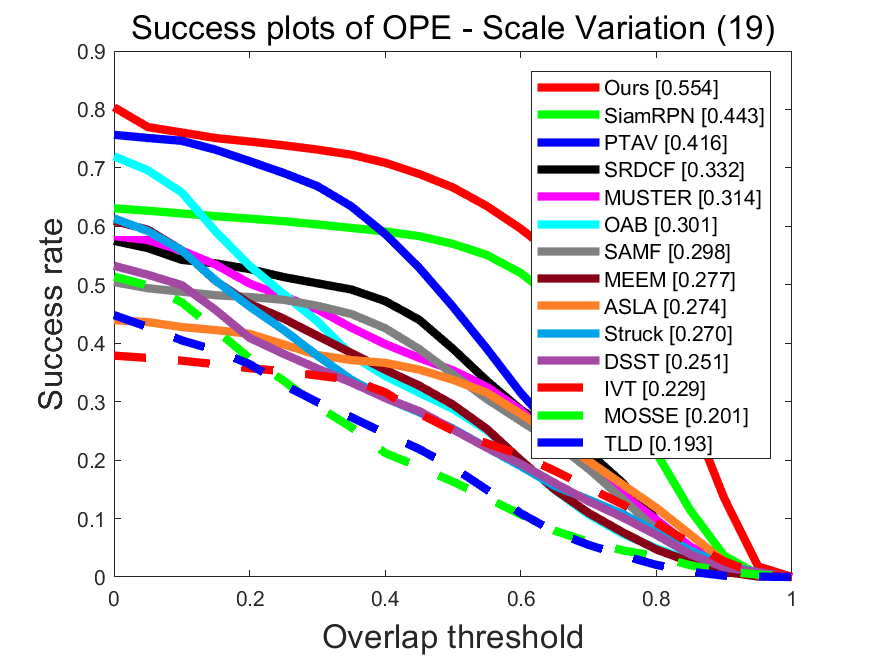
\includegraphics[width=0.234\linewidth]
	{images/UAV20L/SV_overlap_OPE_AUC.png}
}
\subfigure[]{
	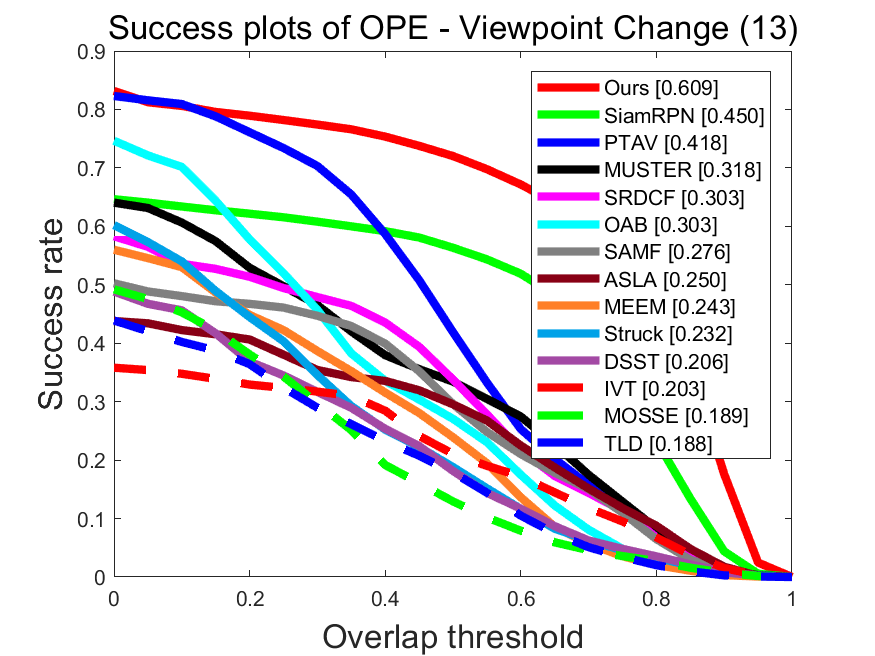
\includegraphics[width=0.234\linewidth]
	{images/UAV20L/VC_overlap_OPE_AUC.png}
}
\end{center}
   \caption{Success plots with attributes on UAV20L. Best viewed on color display.}
\label{fig:uav20l_attr}
\end{figure*}
\fi

UAV20L \cite{mueller2016benchmark} 是从低空空中视角捕获的空中视频数据集。 UAV20L数据库专为长期跟踪而设计,包含20个视频,平均长度为2934帧。
遵循OTB50 \cite{OTB}的评估方法,我们使用精度和成功度来评估UAV20L数据集上跟踪器的性能。精度是指从预测边界框的中心点到地面真值边界框的中心点的距离。成功是指预测边界框与地面真值边界框的并集​​(IOU)交集。在图 \ref{fig:uav20l}中,不同跟踪器的性能比较通过精度图和成功图可视化。

将该方法与最近的13种追踪器进行了比较。图 \ref{fig:uav20l} 清楚地表明,我们的算法在成功率和精确度得分方面均胜过所有其他跟踪器。具体来说,在成功图中,我们的跟踪器获得的AUC得分为0.557。与最先进的方法 PTAV \cite{fan2018parallel} 和 SiamRPN \cite{SiamRPN}相比,拟议的跟踪器的性能要优于这些跟踪器,分别为31.7%和22.7%。在精度图中,所提算法的得分为0.776。与 SiamRPN \cite{SiamRPN} 和 PTAV \cite{fan2018parallel}相比,拟议的跟踪器相对于这些跟踪器的性能分别高 25.8\% 和 24.4\%。

\iffalse
In order to perform a more in-depth and detailed analysis of the performance of the trackers, we also report the results on challenging attributes in UAV20L. Fig. \ref{fig:uav20l_attr} lists the success plots of 14 different methods on 12 attributes: ARC (Aspect Ratio Change), BC (Background Clutter), CM (Camera Motion), FM (Fast Motion), FOC (Full Occlusion), IV (Illumination Variation), LR (LR Low Resolution), OV (Out-of-View), POC (Partial Occlusion), SOB (Similar Object), SV (Scale Variation) and VC (Viewpoint Change). We can observe that the AUC of the proposed algorithm perform better than other methods on most challenging attributes, which means our method is more robust than other approaches on various difficult situations.
\fi

\section{结论}
\label{sec:conclusion}

在本文中,我们提出了一种新颖的跟踪体系结构,其中包括跟踪组件和数据驱动的运动模型。全局感知机制允许跟踪组件减少跟踪过程中的累积错误。跟踪组件使用非常深的网络进行两阶段跟踪,这使跟踪器更具区分性。运动模型是端到端训练的,并且能够从大规模轨迹数据集中学习目标的运动模式。通过跟踪组件和运动模型的协同工作,所提出的方法对最新的跟踪器具有良好的性能。